\section{Subtipado}
Muchos lenguajes nos ofrecen la posibilidad de trabajar con subtipos. Esto significa que definen una relación entre sus tipos que, en ciertos casos, nos permite usar a un elemento de un tipo como si fuese un elemento de otro.  Por ejemplo, si tenemos una función que toma dos $Float$ (reales) y nos devuelve su suma, a esa función podriamos pasarle un $Nat$ (natural) o un $Int$ (entero) y podríamos ejecutarla sin problema ya que estos tipos, en realidad, son subconjuntos de los reales.

Hasta ahora, para nuestro lenguaje $\lambda$, definimos un sistema de tipado que descarta todos los programas que no tipen, sin embargo la definición de tipado que tenemos es demasiado rígida y no nos permite definir programas con este estilo. Por esta razón, vamos a extender nuestro sistema y definir nuevas reglas de tipado que nos permitan incluir este tipo de expresiones en el conjunto de expresiones tipables del lenguaje.

\paragraph{Principio de sustitutividad}
Primero definimos la relación $\sigma <: \tau$, que indica que en todo contexto donde se espera una expresión de tipo $\tau$, podemos utilizar una de tipo $\sigma$ en su lugar \textbf{sin} que ello genere un error. Y además agregamos la regla de subtipado (\textbf{Subsumption}) T-Subs:
$$\frac{\judgeType{\Gamma}{M}{\sigma}~\hspace*{5mm}~\sigma <:\tau}{\judgeType{\Gamma}{M}{\tau}}(\text{T-Subs})$$

Esta regla es la que nos dice que si tenemos una expresión de tipo $\sigma$ tal que $\sigma <: \tau$, entonces también podremos considerar a $M$ como una expresión de tipo $\tau$.
\paragraph{El tipo máximo}  Además, vamos a agregar, a nuestro lenguaje, el tipo $Top$ que contendrá a todos los tipos del lenguaje y lo llamaremos \textbf{supertipo universal} porque todo tipo es subtipo de $Top$:
$$\frac{}{\sigma <: Top}(S-Top)$$

\paragraph{Tipos con constructores invariantes:} Son aquellos tipos que no pueden ser remplazados por ningún otro.

\paragraph{Tipos con constructores covariantes:} Son aquellos que tipos cuyo subtipos se consiguen remplazando sus argumentos por un subtipo del argumento.

\paragraph{Tipos con constructores contravariantes:} Son aquellos que tipos cuyo subtipos se consiguen remplazando sus argumentos por un supertipo del argumento.


\subsection{Reglas de subtipado}
\subsubsection{Tipos básicos}
\begin{align*}
\frac{}{Nat <: Float}(\text{S-NatFloat}) \hspace*{5mm}\frac{}{Int <: Float}(\text{S-IntFloat}) \hspace*{5mm}\frac{}{Bool <: Nat}(\text{S-BoolNat})
\end{align*}


\subsubsection{Subtipado del tipo función}
Buscamos una función $g:\sigma\to\tau$ que pueda remplazar a otra función $f:\sigma'\to\tau'$ en cualquier contexto sin generar ningún error. 
Lo primero que tenemos que tener en cuenta es que $g$ debe estar definida para todos los elementos del dominio de $f$, osea $Dom(f)\subseteq Dom(g)$ pues si pasara que existe un valor $x$ tal $f(x)$ está definida y $g(x)$ no lo está, entonces obtendríamos un error. Entonces, $\sigma' <: \sigma$.

Por otro lado, $g$ no debería poder devolver como resultado ningún valor que no esperamos que $f$ no devuelva ($Im(g)\subseteq Im(f)$). Podemos aclarar esto con un ejemplo, supongamos que tenemos la función $\text{esPar} :: Nat\to Nat$, cuando usemos esta función, el contexto en el que la usemos estará esperando conseguir un natural de su evaluación. Si la función $g$ devuelve algo que no sea un $Nat$, entonces obtendriamos un error. Sin embargo, si $g :: Nat\to Bool$, entonces podremos realizar el remplazo sin ningún problema porque $\{0,1\}$ es un subconjunto de los naturales. Luego $\tau <: \tau'$.

Y la regla de subtipado queda:

\vspace*{5mm}
$$\frac{\sigma' <: \sigma\hspace*{5mm}\tau <: \tau'}{\sigma\to\tau <: \sigma'\to\tau'}(\text{S-Func})$$

\vspace*{5mm}
El constructor de tipos función es \textbf{contravariante} en su primer argumento y \textbf{covariante} en el segundo.

Un programa $P$, deberá \textbf{coercionar} (transformar) el argumento que le pasan a la función para que coincida con el tipo de la nueva función, ejecutarla y luego coercionar su resultado al tipo del resultado que espera $P$.

\subsubsection{Reglas de subtipado de términos}
Las reglas de tipado sin subtipos son dirigidas por sintaxis, por lo que es inmediato implementar un algoritmo de chequeo de tipos a partir de ellas. Con el agregado de la regla T-Subs, el chequeo también pasa a estar dirigidas por la semántica de la relación $<:$, por lo que el algoritmo deja de ser tan directo.

Un juicio de subtipado $\judgeTypeS{\Gamma}{M}{\sigma}$, nos dice que $\judgeType{\Gamma}{M}{\sigma}$ y que existe existe $\tau$ tal que $\judgeTypeS{\Gamma}{M}{\tau}$ con $\tau <: \sigma$. Entonces las nuevas reglas quedarían así:

\begin{equation*}
\begin{gathered}
    \frac{x:\sigma\in\Gamma}{\judgeTypeS{\Gamma}{x}{\sigma}}(\text{T-Var})\hspace*{2cm}
\vspace*{5mm} \\
    \frac {\judgeTypeS{\Gamma,x:\sigma}{M}{\tau}}
          {\judgeTypeS{\Gamma}{\lambdaAbs{x}{\sigma}{M}}{\sigma\to\tau}}(\text{T-Abs})\hspace*{2cm}
    \frac{\judgeTypeS{\Gamma}{M}{\sigma\to\tau}\hspace*{5mm}\judgeTypeS{\Gamma}{N}{\blue{\rho}}\hspace*{5mm}\blue{\rho <: \sigma}}{\judgeTypeS{\Gamma}{M~N}{\tau}}(\text{T-App})
\end{gathered}
\end{equation*}

La mayoría de las reglas de subtipado son similares a las reglas de tipo y la  única regla que usa la relación $<:$ de manera explicita es T-App, porque los términos de aplicación son los únicos que al ser evaluados remplazan expresiones y, efectivamente, esta regla es la que nos da el poder que estabamos buscando.


\subsubsection{Relación de preorden} La relación de subtipado $<:$ define una relación de preorden, es decir es reflexiva y transitiva por lo que podriamos escribir las siguientes reglas:

$$\frac{}{\sigma <: \sigma}(\text{S-Refl}) \hspace*{1cm}\frac{\sigma <:\tau\hspace*{5mm}\tau <: \rho}{\sigma <: \rho}(\text{S-Trans})$$

Sin embargo, esta forma de descrbir la relación no es dirigida por semántica y no está claro como hacer un algoritmo de chequeo de subtipos que use estas reglas. Por esta razón vamos a considerar los siguientes tres axiomas:

\begin{align*}
\frac{}{Nat <: Nat}(\text{S-NatNat}) \hspace*{5mm}\frac{}{Bool <: Bool}(\text{S-BoolBool}) \hspace*{5mm}\frac{}{Float <: Float}(\text{S-FloatFloat})
\end{align*}

\vspace*{5mm}
Y ya con eso alcanza para derivar la reflexibidad de cualquier tipo del lenguaje, en el lenguaje $\lambda$ básico. Si agregasemos un nuevo tipo escalar (sin parámetros), entonces debemos declarar explicitamente que ese tipo es subtipo de si mismo, sino el preorden se rompe.

Por otro lado, la transitividad se puede demostrar aplicando varios pasos de subtipado, por lo que directamente no es necesaria.

\subsubsection{Algoritmo de chequeo de tipos}
Entonces logramos escribir todas las reglas del sistema de subtipado de manera tal que son dirigidas por la sintaxis y podemos definir el algoritmos $subtype(S,T)$ que nos indica si $S$ es subtipo de $T$. Al algoritmo mostrado le faltan los axiomas de $Nat$, $Bool$ y $Float$ que son triviales (hay que poner cada una de esas comparaciones una por una):

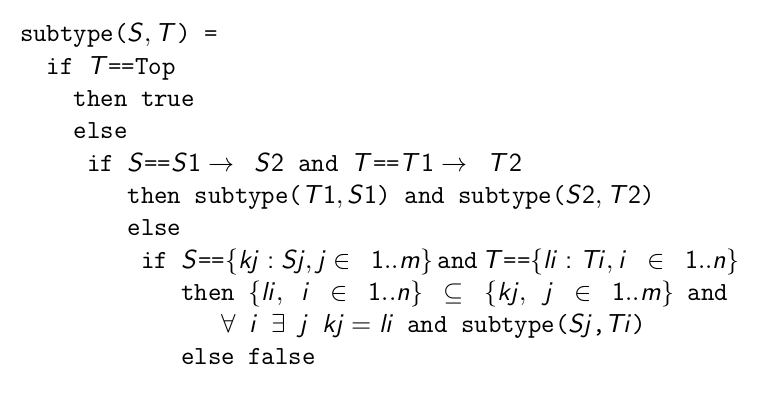
\includegraphics[scale=0.4]{imagenes/algoritmo_subtipado.png}

\subsection{Subtipado de referencias}
Queremos encontrar el tipo $Ref~\tau$ que sea subtipo de $Ref~\sigma$. Supongamos que $\tau <: \sigma$, si intentamos subtipar una referencia $M:Ref~\sigma$ con $Ref~\tau$, entonces cuando realicemos una asignación podremos usar un valor de tipo $\tau$ y no tendremos error. Ahora, cuando derreferenciemos $M$ estarémos esperando algo de tipo $\sigma$, pero como $\tau$ es más general que $\sigma$ puede tener valores que no son de ese tipo, por lo que si un contexto esperaba algo del primer tipo se obtendría un error.

Si  $\sigma <: \tau$ y $M: Ref~\sigma$, entonces podemos guardar en $M$ un elemento de tipo $\sigma$, sin embargo cuando querramos derreferenciar $M$, como $Ref~\sigma$ es subtipo de $Ref~\tau$, podremos usar la derreferencia del segundo tipo. El problema vuelve a ser el mismo, el contexto va a estar esperando un valor de tipo $\tau$, pero $\sigma$ es más general, por lo que el valor almacenado en $M$ puede no ser de este tipo, lo que llevaría a un error.

A continuación dos ejemplos que muestran cada caso usando los tipos $Int <: Float$:
\begin{align*}
&\lambdaLetI{r}{\text{ref}~3}{r := 2.1}; \\
&!r
\end{align*}
Este es el primer caso, como definimos $r$ como una referencia de enteros en el let, cuando derreferenciemos $r$ esperamos conseguir un entero, sin embargo la regla covariante, hace que con la asignación podamos asignar a $r$ un $Float$

\begin{align}
\lambdaLetI{r}{\text{ref}~2.1}{!r}
\end{align}

Y este es el segundo caso, en el que definimos a $r$ como una referencia de $Float$, sin embargo, como $r$ es subtipable a $Ref~Int$, podemos usar la derreferenciación de enteros para derreferenciarla, lo que provocaría el error en el programa.

Entonces, la regla de subtipado no es ni contravariante ni covariente, es variante. La única ``sustitución" que podemos hacer es cuando $\sigma$ y $\tau$ son el mismo tipo.

$$\frac{\sigma <: \tau\hspace*{5mm} \tau <: \sigma}{Ref~\tau <: Ref~\sigma}$$

\subsubsection{Refinando el tipo \textit{Ref}}
Extendemos el lenguaje, con los siguiente tipos $Source~\sigma$ y $Sink~\sigma$ que representan las referencias de lectura y las de escritura, respectivamente. 

\paragraph{Reglas de tipado}

\begin{align*}
\frac{\judgeType{\Gamma|\Sigma}{M}{Source~\sigma}}{\judgeType{\Gamma|\Sigma}{!M}{\sigma}}(\text{T-DeRefSource})
\end{align*}

\begin{align*}
\frac{\judgeType{\Gamma|\Sigma}{M}{Sink~\sigma}\hspace*{5mm} \judgeType{\Gamma|\Sigma}{N}{\sigma}}{\judgeType{\Gamma|\Sigma}{M := N}{Unit}}(\text{T-AssignSink})
\end{align*}

\paragraph{Reglas de subtipado}
\begin{align*}
\frac{\sigma <: \tau}{Source~\sigma <: Source~\tau}(\text{S-Source})\hspace*{1cm}\frac{\tau <: \sigma}{Sink~\sigma <: Sink~\tau}(\text{S-Sink})
\end{align*}

\begin{align*}
\frac{}{Ref~\tau <: Source~\tau}(\text{S-RefSource})\hspace*{1cm}\frac{}{Ref~\tau <: Sink~\tau}(\text{S-RefSink})
\end{align*}
La regla S-Source es covariante, si esperamos leer de una referencia de tipo $\tau$, entonces podemos esperar una referencia de un tipo más especifico que $\tau$. 

La regla S-Sink es contravariante, ya que cuando querramos guardar un valor de tipo $\tau$, podremos guardarlo en una referencia de este tipo o en una de un tipo más general.

Además, $Source~\tau$ y $Sink~\tau$ son mas generales que $Ref~\tau$ ya que siempre podremos remplazar referencias de lecturas o de escritura por referencias de lectura y escritura.